%%% Local Variables:
%%% mode: latex
%%% TeX-master: t
%%% End:

\newpage

\subsection{Sequence Diagram}

A sequence diagram or system sequence diagram (SSD) shows process interactions arranged in time sequence in the field of software engineering. It depicts the processes involved and the sequence of messages exchanged between the processes needed to carry out the functionality.

The following diagram shows the interaction between the user, dApp, blockchain, web3 provider, and IPFS network.

\namedfigure
{!hbtp}
{img:connectSeqDig}
{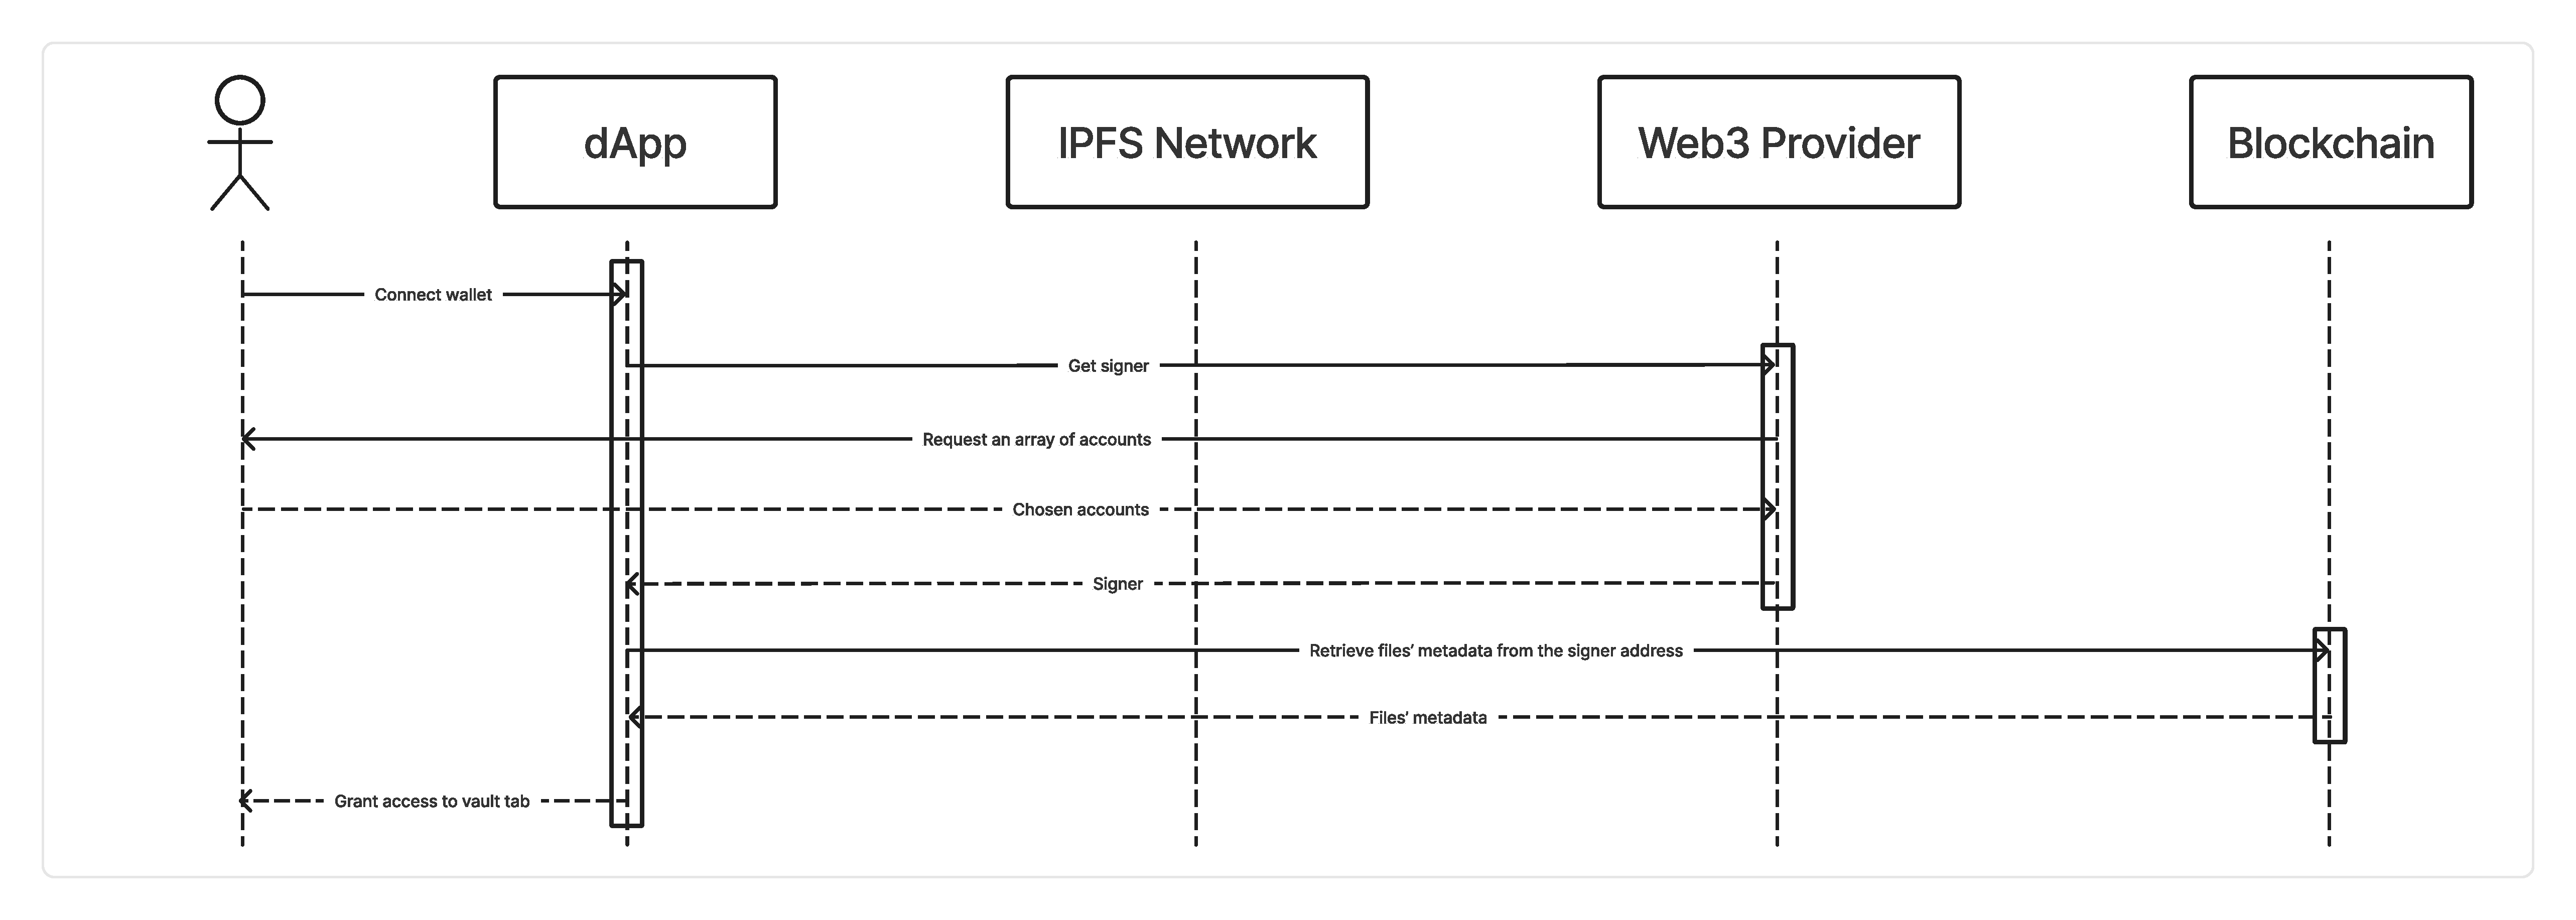
\includegraphics[width=\textwidth]{connect_seq_dig.pdf}}
{Connect wallet act in sequential order.}

\namedfigure
{!htbp}
{img:uploadSigDig}
{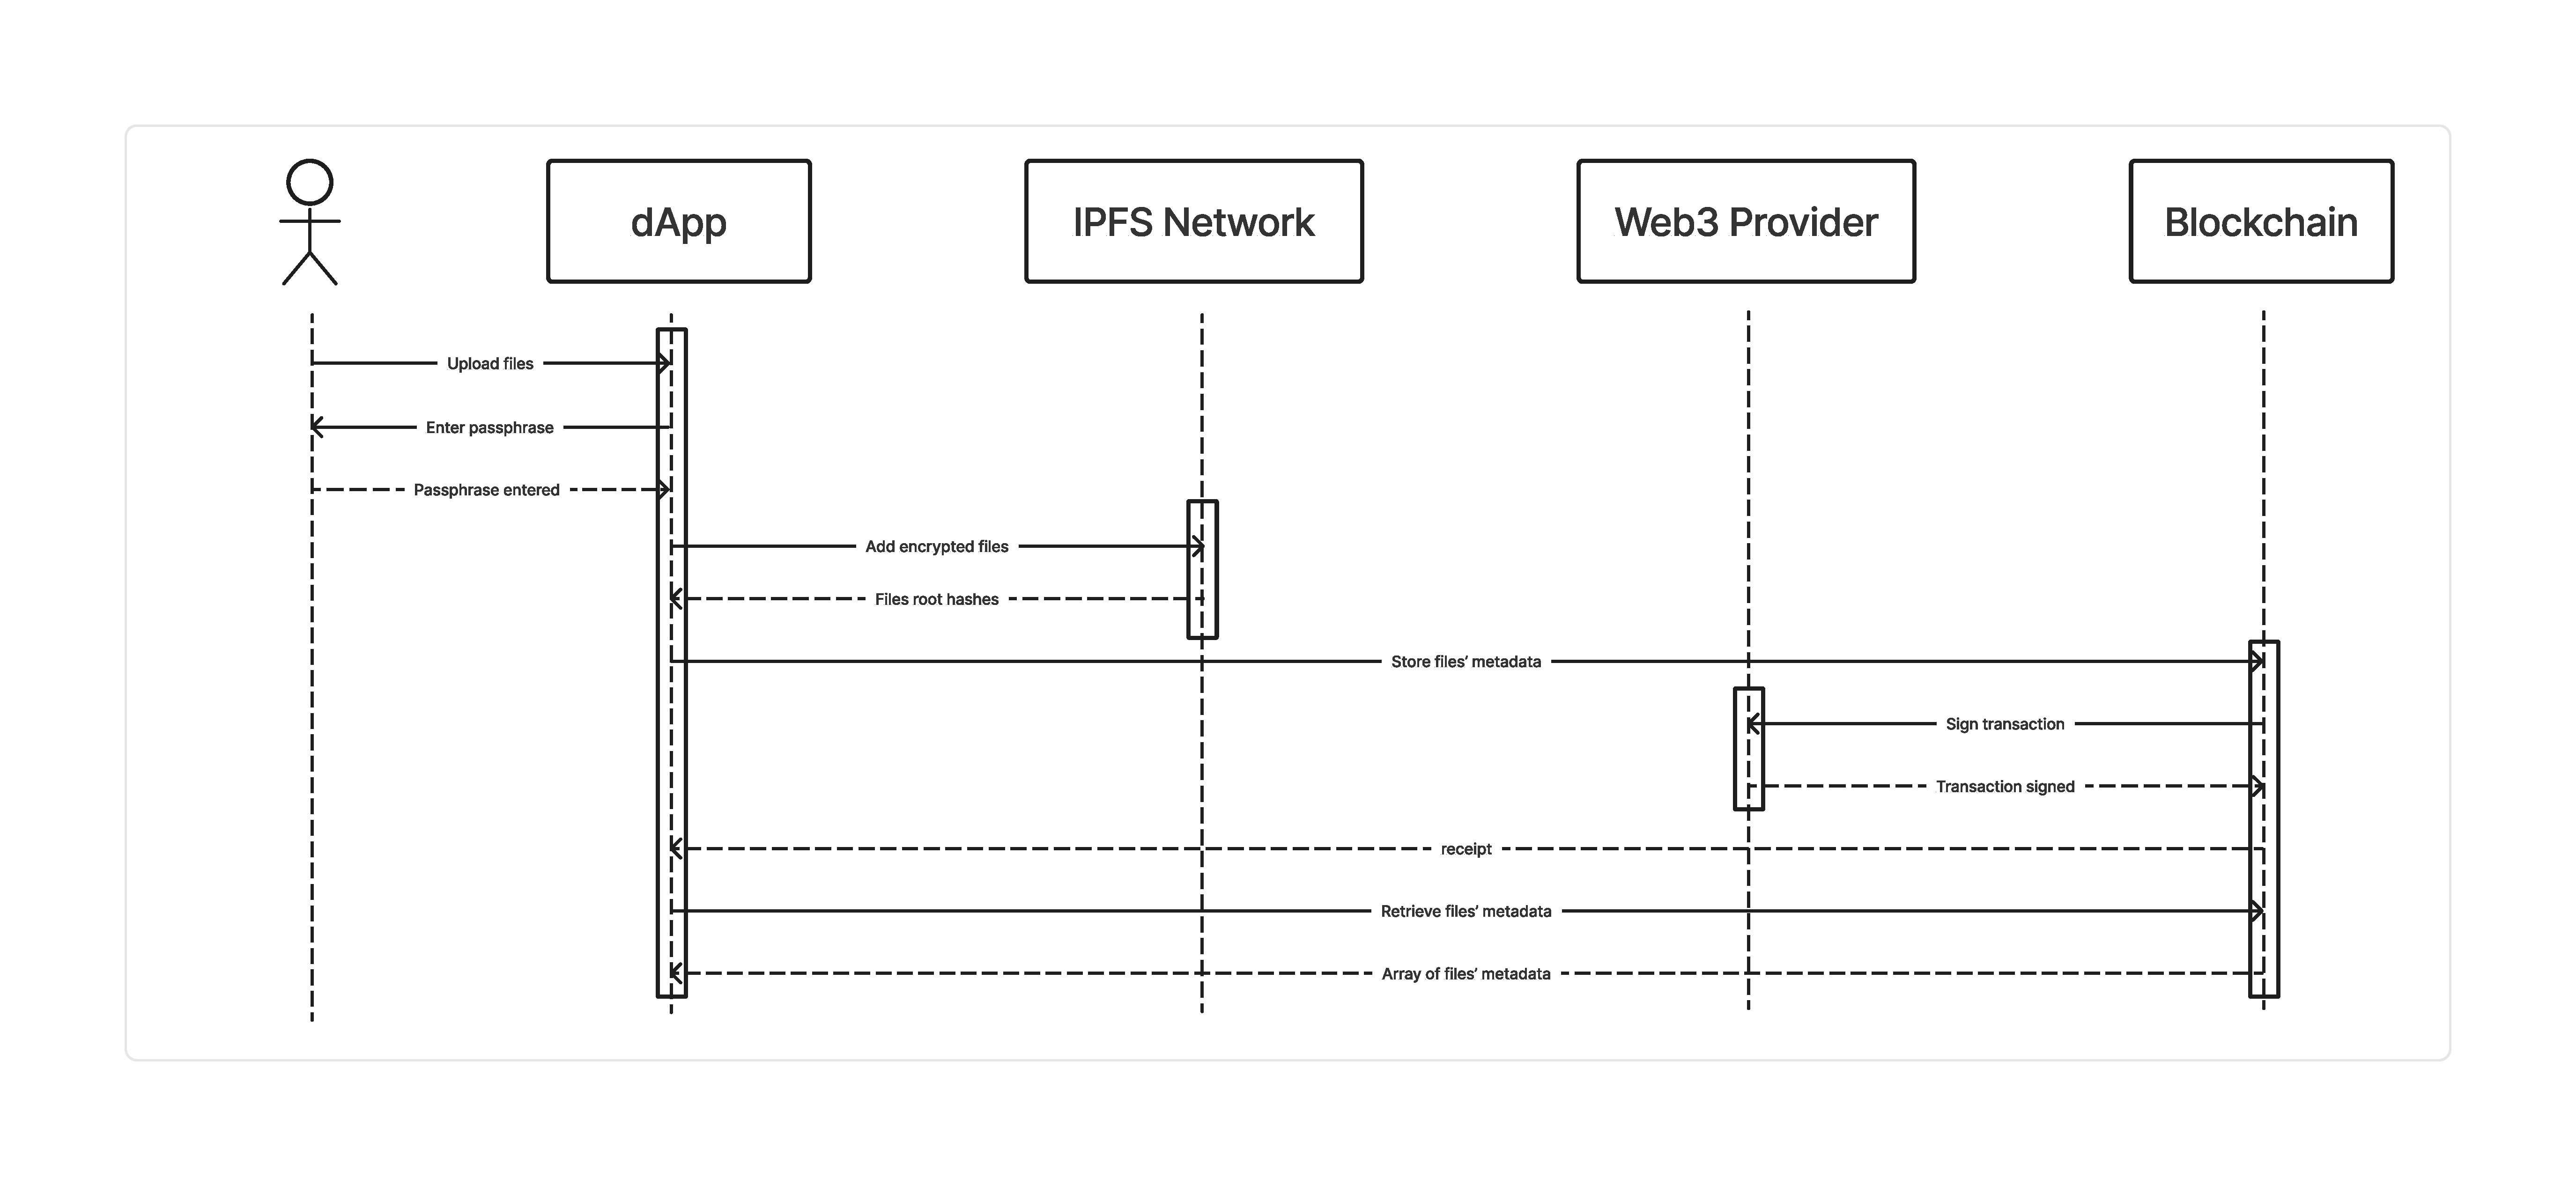
\includegraphics[width=\textwidth]{upload_files_seq_dig.pdf}}
{Upload files act in sequential order.}

\namedfigure
{!hbtp}
{img:downloadSigDig}
{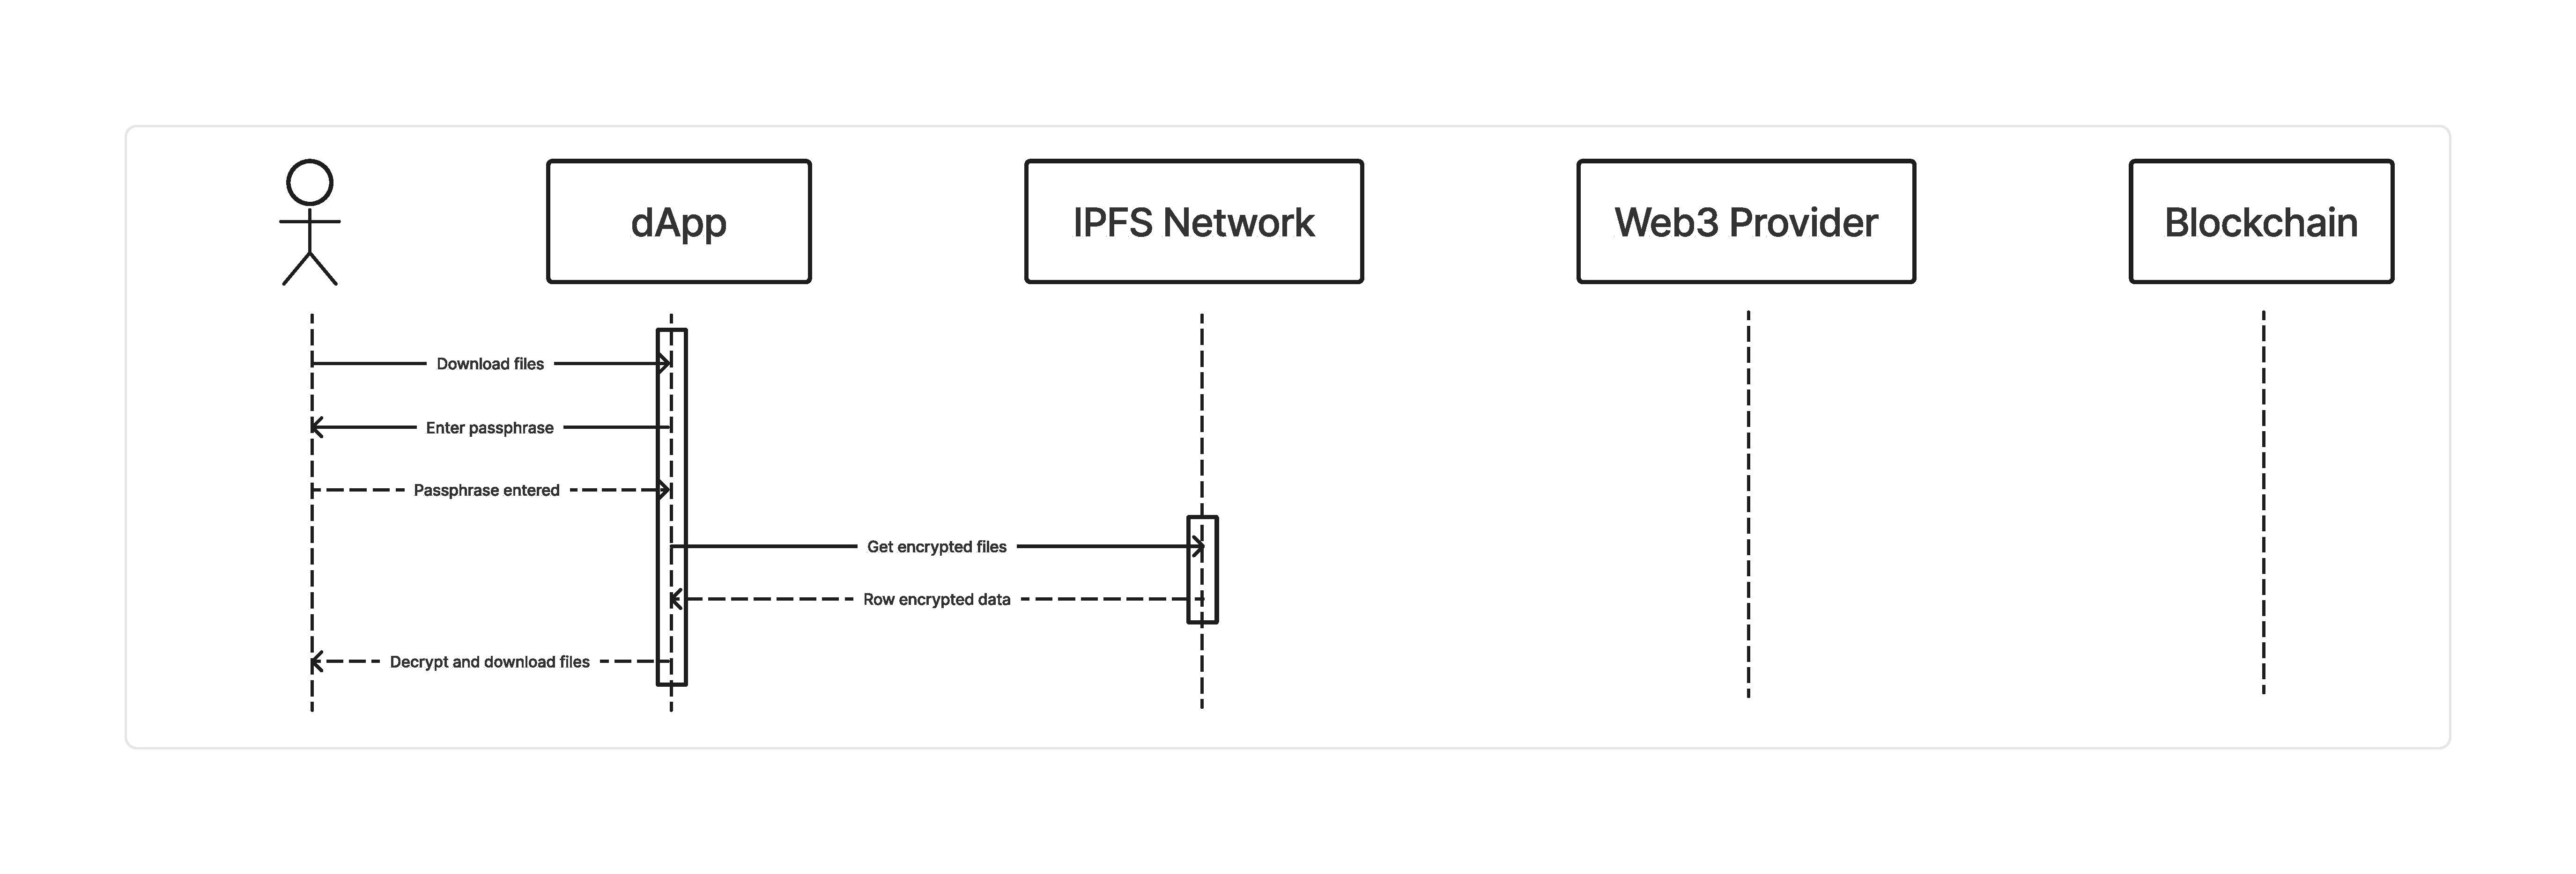
\includegraphics[width=\textwidth]{download_files_seq_dig.pdf}}
{Download files act in sequential order.}

\namedfigure
{!htbp}
{img:shareSigDig}
{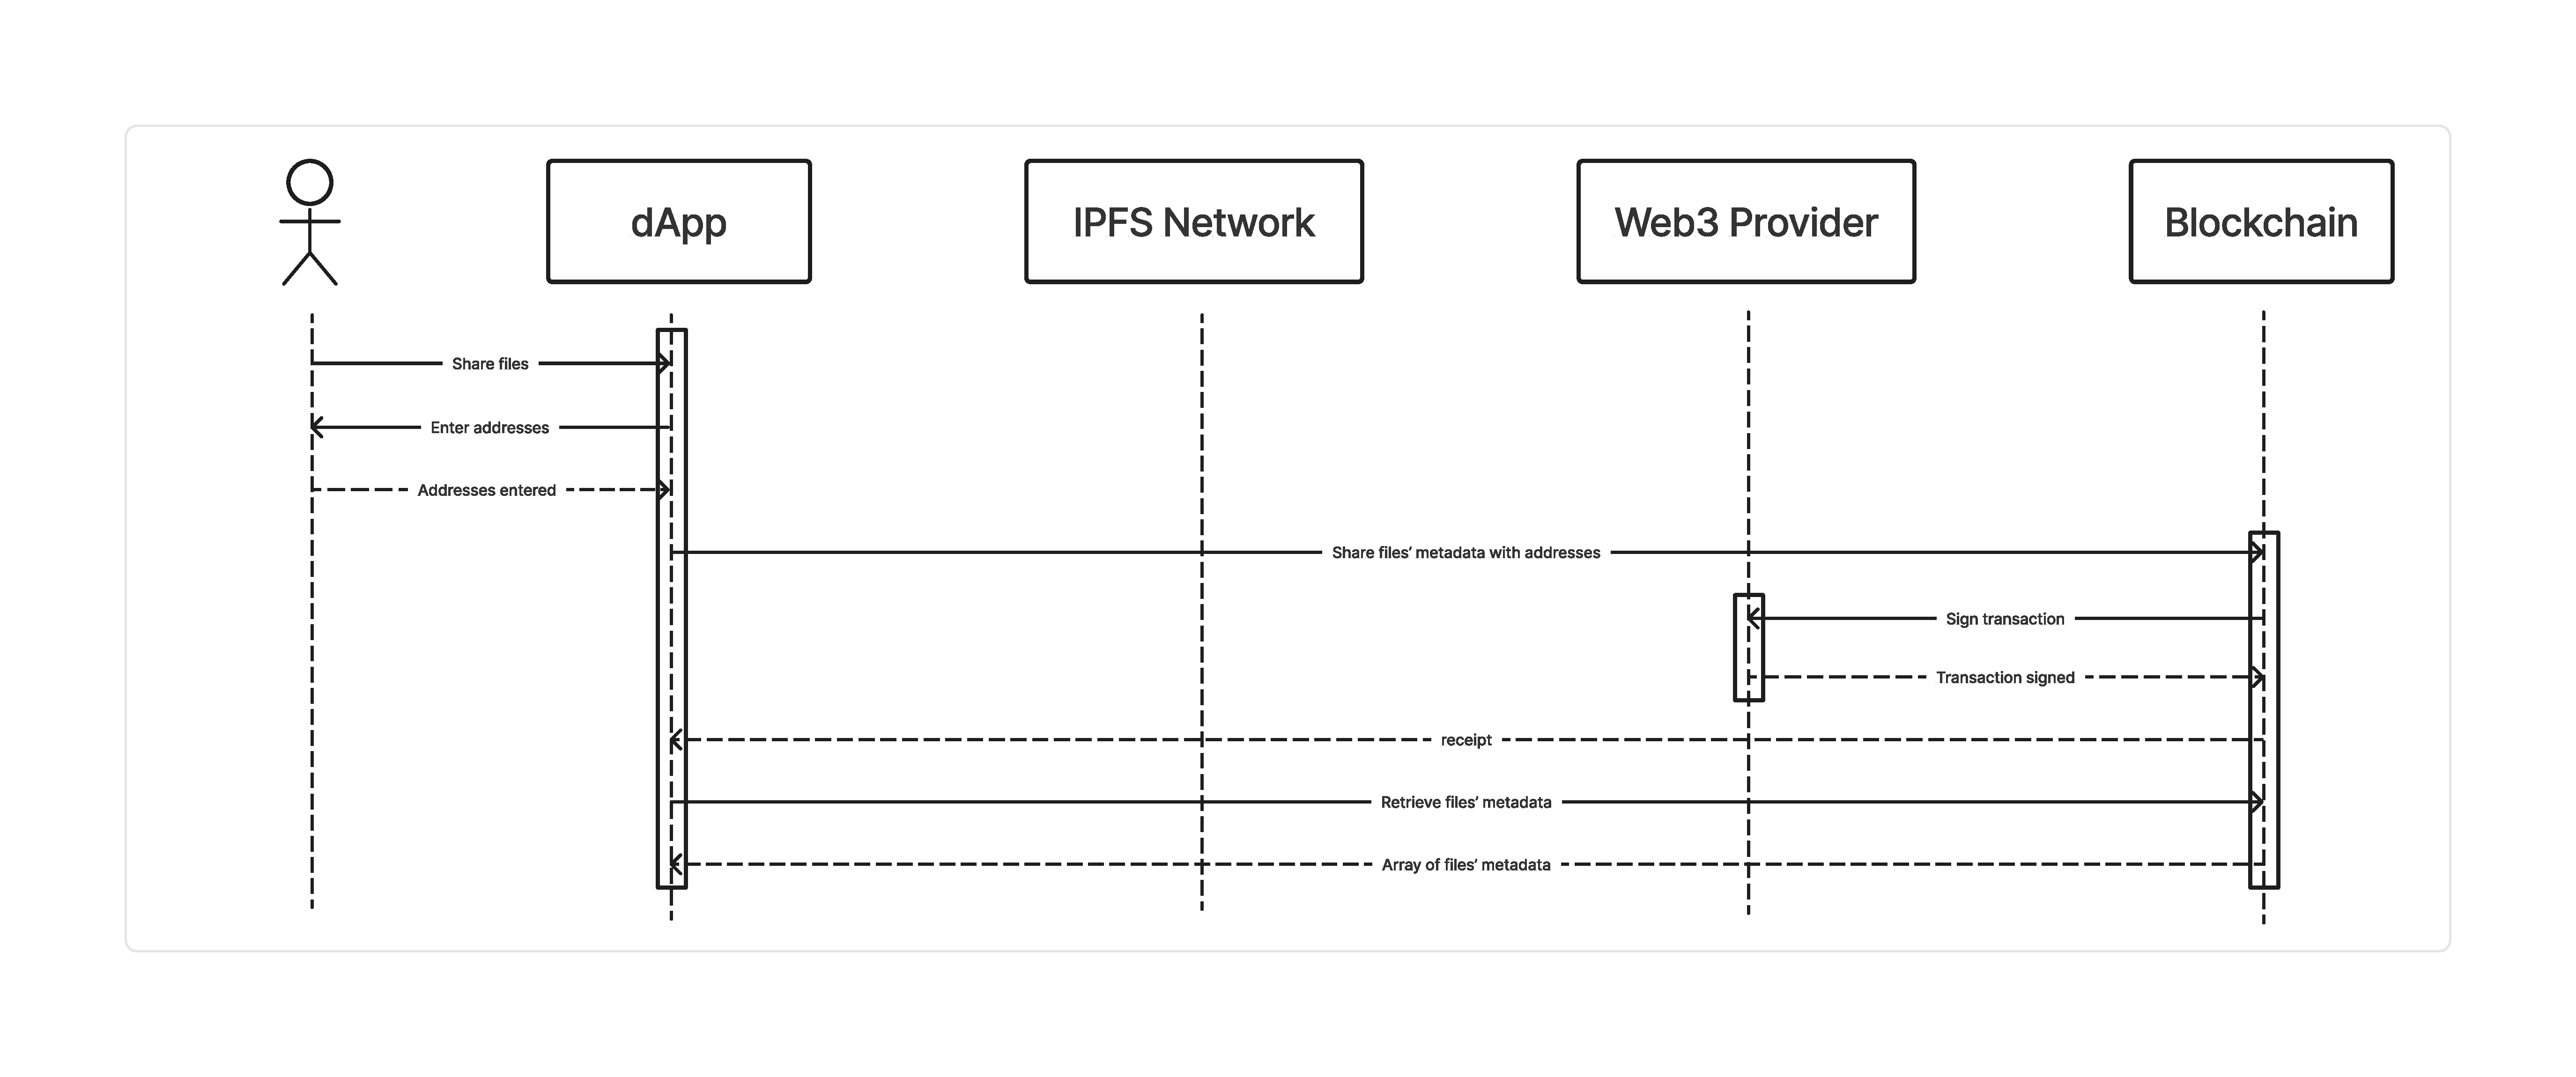
\includegraphics[width=\textwidth]{share_files_seq_dig.pdf}}
{Share files act in sequential order.}

\namedfigure
{!hbtp}
{img:deleteSigDig}
{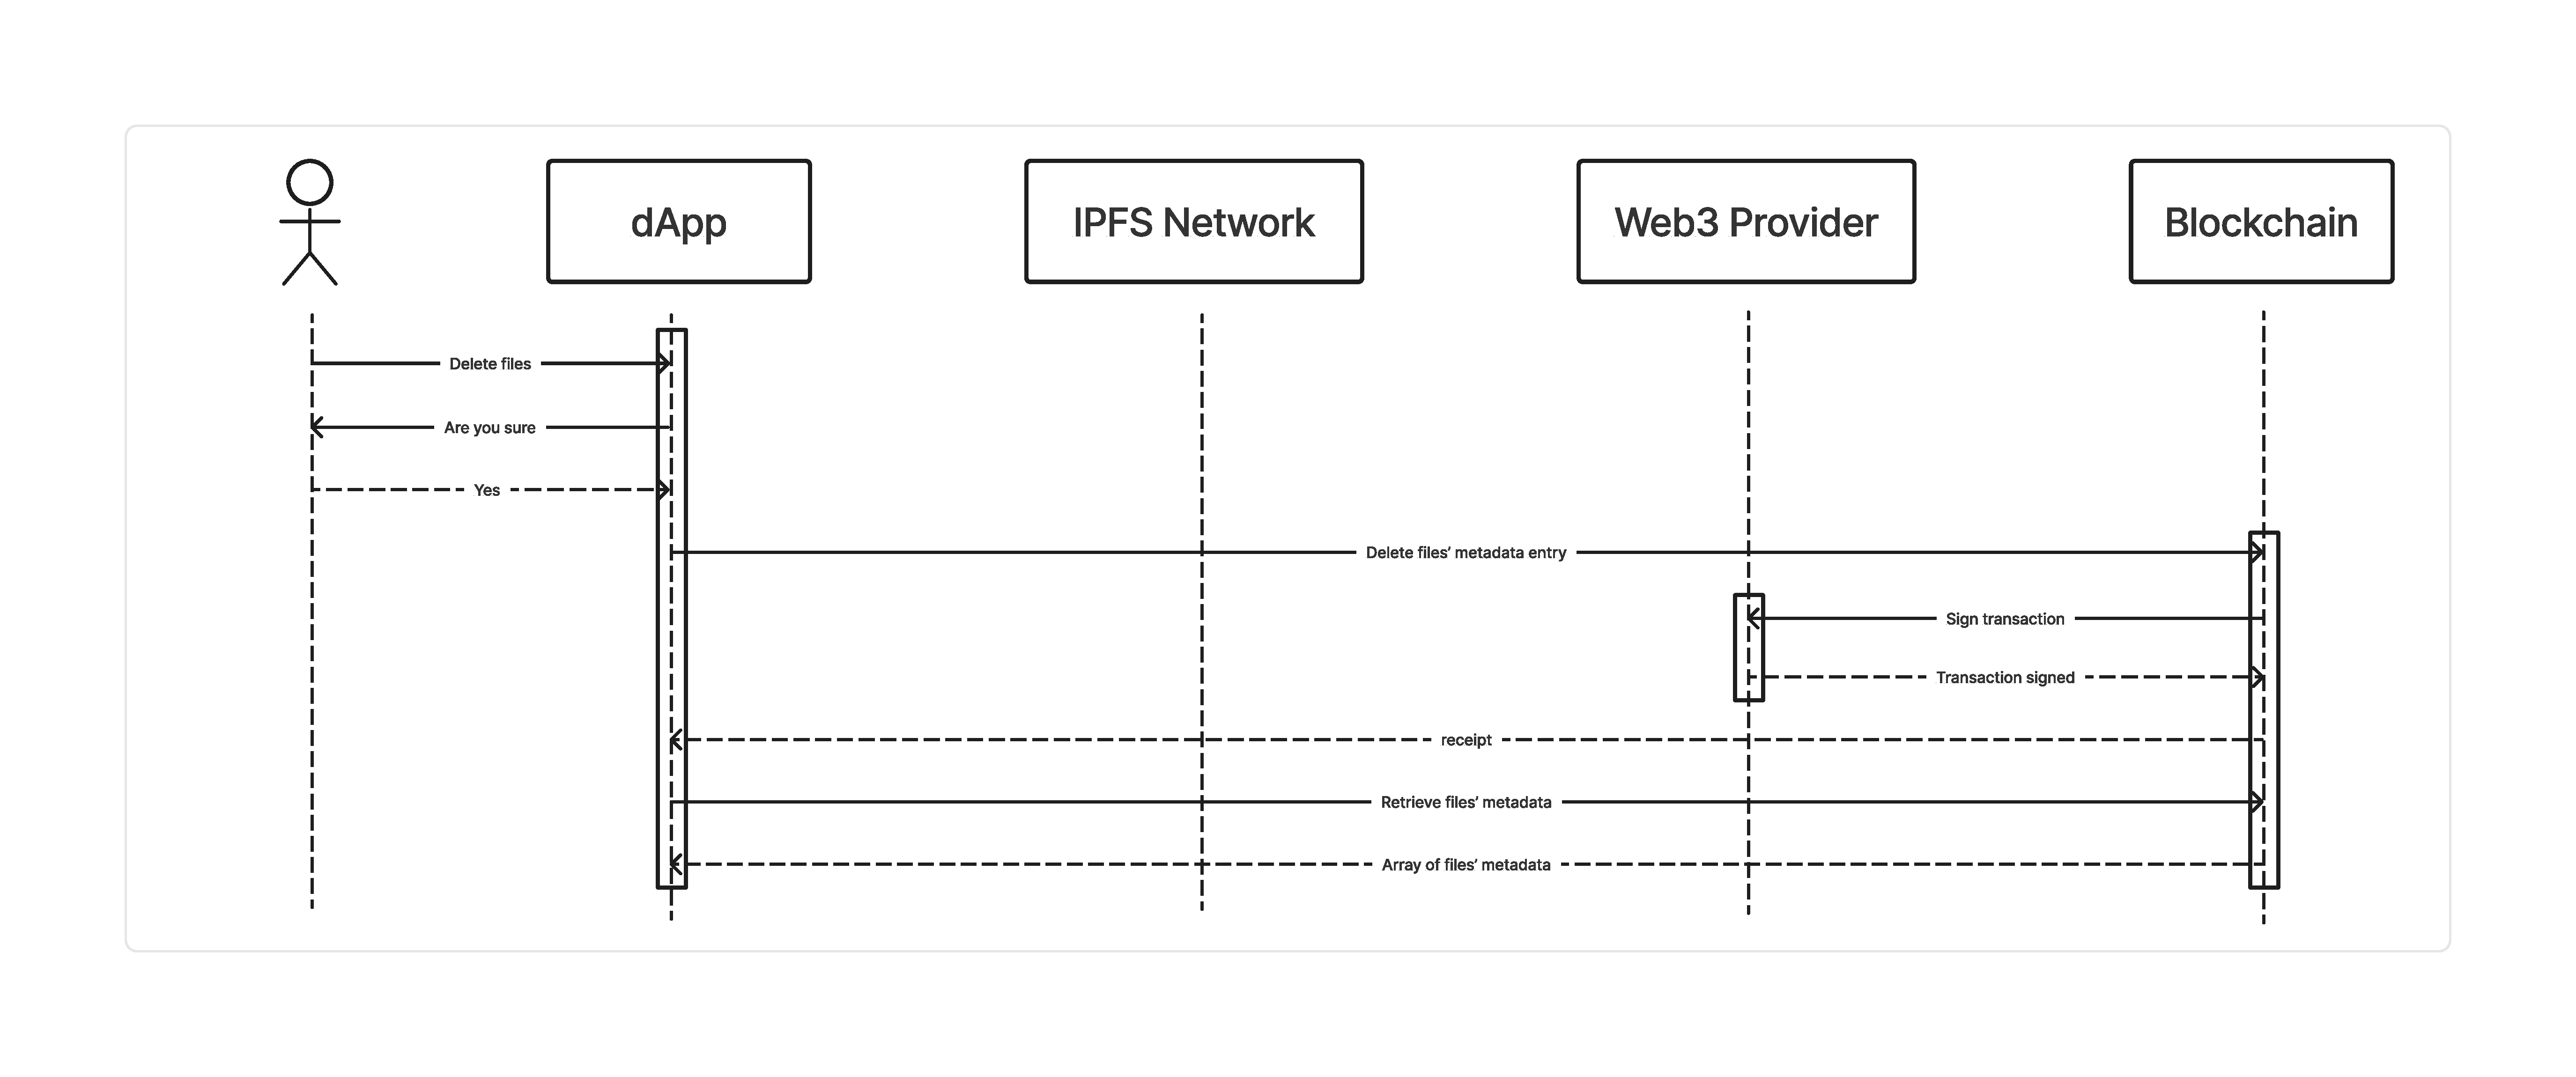
\includegraphics[width=\textwidth]{delete_files_seq_dig.pdf}}
{Delete files act in sequential order.}
